\subsubsection{Guidance method's questionnaire.}
\label{subsubsec:results_questionnaires_2}

The Figure \ref{fig:boxplot_questionnaire_scene} presents the box plot with the distribution of the scores. It is possible to see that there is some similarity between the two groups, except for the virtual cane method, which has a broader distribution for the sighted users. Also, it seems that the audio and mixture have similar acceptance for sighted and blind users.

\begin{figure}[!htb]
    \centering
    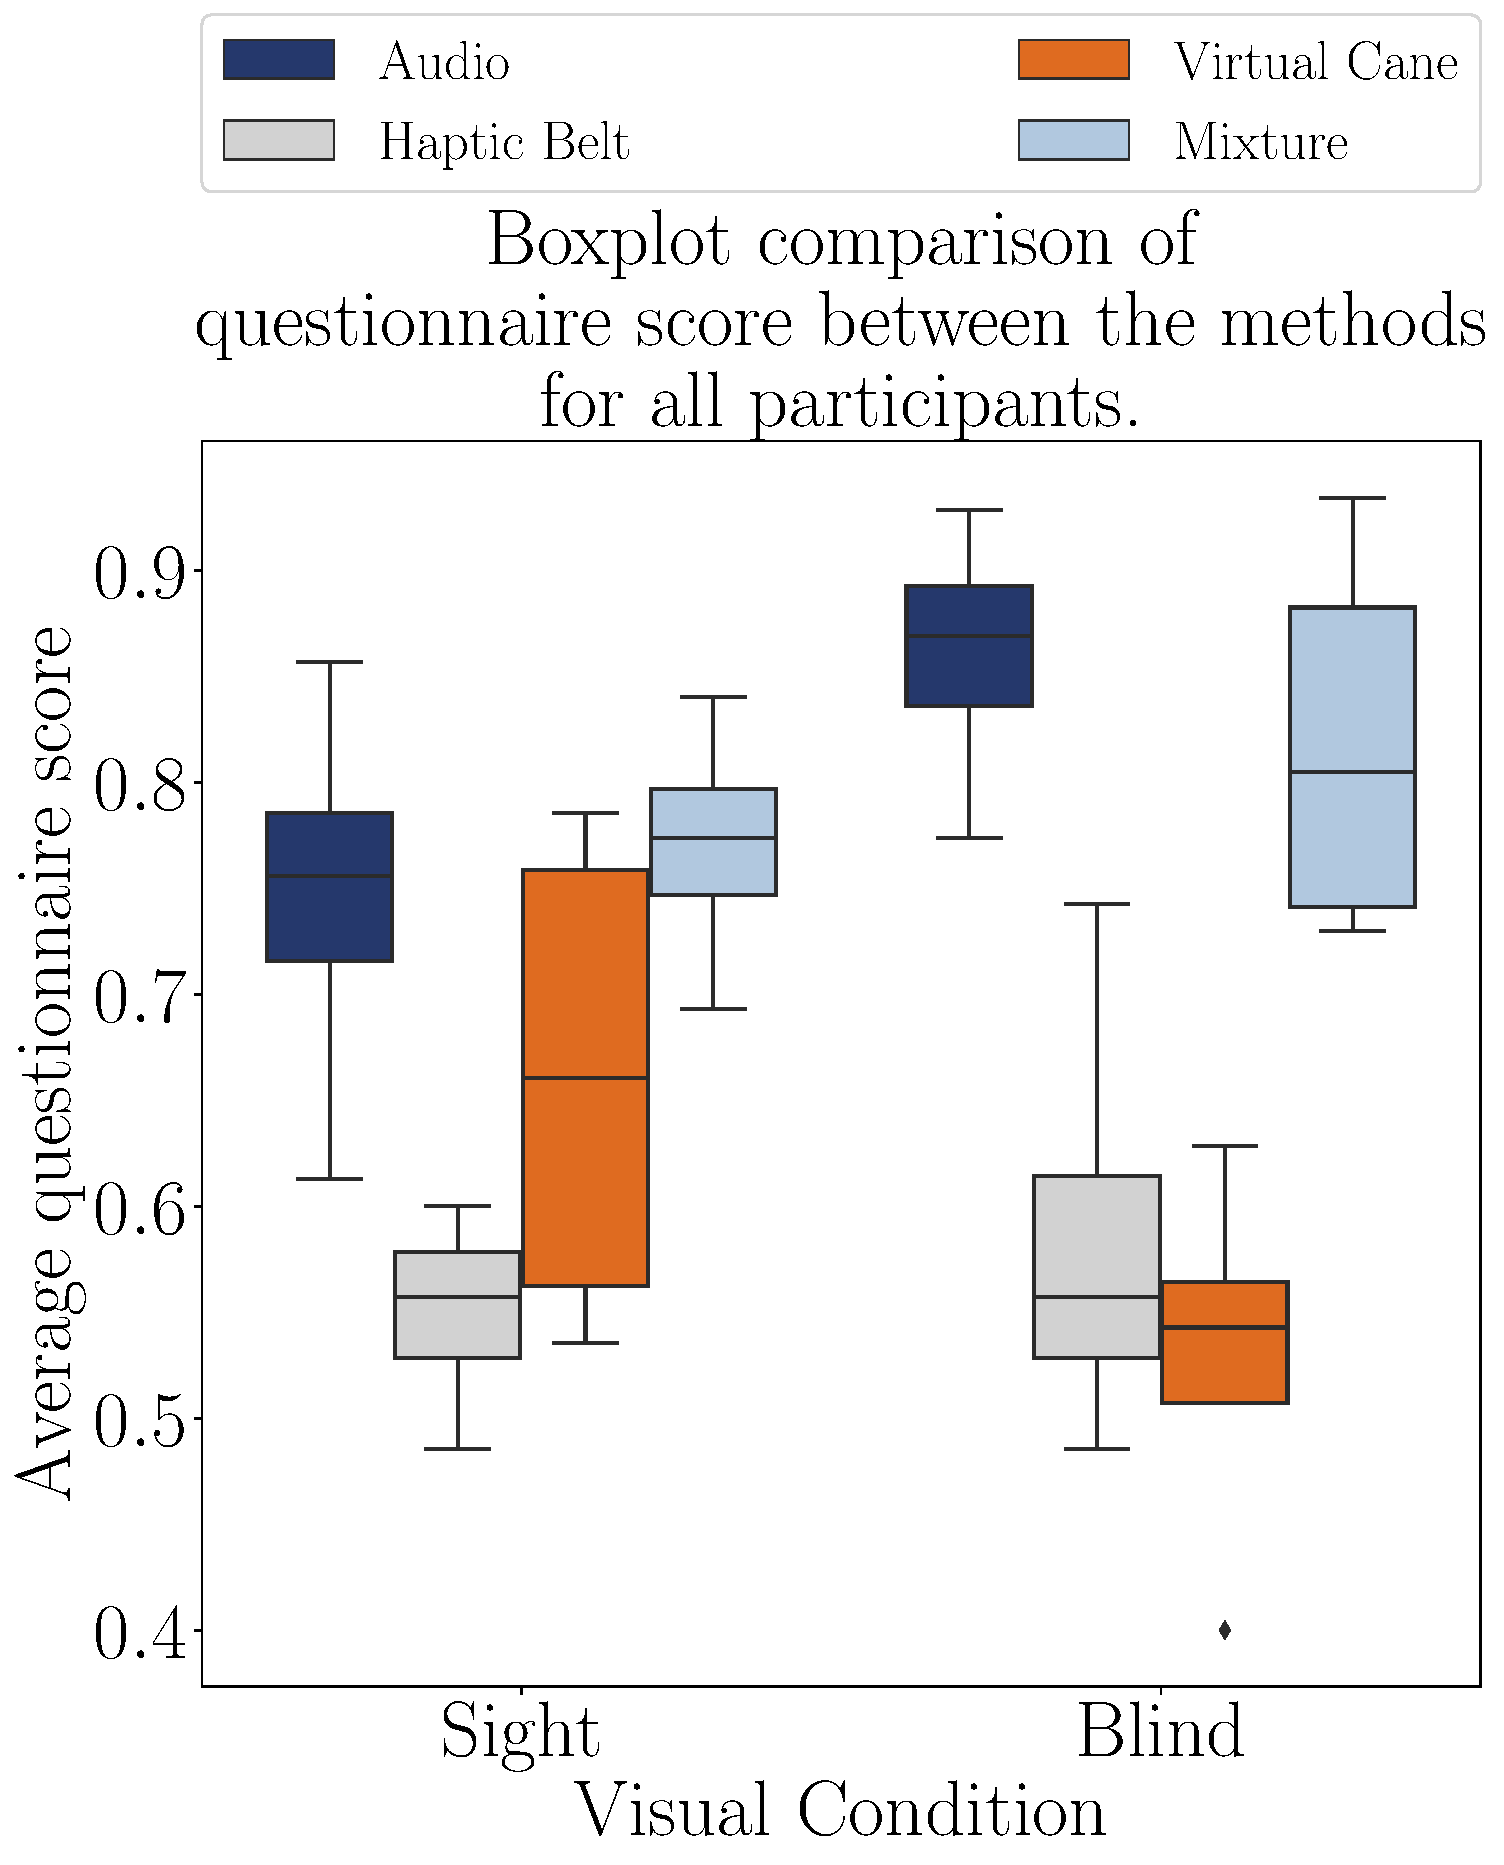
\includegraphics[width = 0.75\linewidth]{3 - Resultados/Figuras/boxplot_questionnaire_scene.pdf}
    \caption{Boxplot of the questionaire score of the the participants grouped by the methods.}
    \label{fig:boxplot_questionnaire_scene}
\end{figure}

The result of ANOVA is presented in Table \ref{tab:blocanova_questionnaire_blind_sight} and indicates that the method is an effective variable for the sighted participants, as it is for the blind ones.

\begin{table}[!htb]
    \caption{Anova p-value for the questionnaire score on each method}
    \label{tab:blocanova_questionnaire_blind_sight}
\begin{minipage}{0.45\linewidth}
    \subcaption{Blind participants.}
    
\centering
\begin{tabular}{ll}
\toprule
Source & P-Value \\
\midrule
Method & 0.001** \\
\bottomrule
\end{tabular}

\end{minipage}%
\begin{minipage}{0.05\linewidth}
\end{minipage}%
\begin{minipage}{0.45\linewidth}
    \subcaption{Sight participants.}
    
\centering
\begin{tabular}{ll}
\toprule
Source & P-Value \\
\midrule
Method & 0.016** \\
\bottomrule
\end{tabular}

\end{minipage}
\end{table}

Table \ref{tab:lsd_questionnaire_blind_sight} presents the conclusion of 
A pairwise Fisher LSD test between all the guidance methods for both groups shows that the results are coincident between the two groups.

%\FloatBarrier

\begin{table*}[!thb]
    \caption{Anova p-value for the mental demand average on each method'}
    \label{tab:lsd_questionnaire_blind_sight}
    \begin{minipage}{1\textwidth}
        \subcaption{Blind participants.}
        
\centering
\begin{tabular}{rcllr}
\toprule
      \multicolumn{3}{c}{Method} &                          \multicolumn{2}{c}{Analysis} \\
\midrule
       Audio & $X$ & Haptic Belt &        $H_1 : \mu_{Audio} \ne \mu_{Haptic Belt}$ & ** \\
      Audio & $X$ & Virtual Cane &       $H_1 : \mu_{Audio} \ne \mu_{Virtual Cane}$ & ** \\
           Audio & $X$ & Mixture &                $H_0 : \mu_{Audio} = \mu_{Mixture}$ &  \\
Haptic Belt & $X$ & Virtual Cane & $H_1 : \mu_{Haptic Belt} \ne \mu_{Virtual Cane}$ & ** \\
     Haptic Belt & $X$ & Mixture &      $H_1 : \mu_{Haptic Belt} \ne \mu_{Mixture}$ & ** \\
    Virtual Cane & $X$ & Mixture &     $H_1 : \mu_{Virtual Cane} \ne \mu_{Mixture}$ & ** \\
\bottomrule
\end{tabular}

    \end{minipage}
    \begin{minipage}{1\textwidth}
        \subcaption{Sight participants.}
        
\centering
\begin{tabular}{rcllr}
\toprule
      \multicolumn{3}{c}{Method} &                          \multicolumn{2}{c}{Analysis} \\
\midrule
       Audio & $X$ & Haptic Belt &        $H_1 : \mu_{Audio} \ne \mu_{Haptic Belt}$ & ** \\
      Audio & $X$ & Virtual Cane &       $H_1 : \mu_{Audio} \ne \mu_{Virtual Cane}$ & ** \\
           Audio & $X$ & Mixture &                $H_0 : \mu_{Audio} = \mu_{Mixture}$ &  \\
Haptic Belt & $X$ & Virtual Cane & $H_1 : \mu_{Haptic Belt} \ne \mu_{Virtual Cane}$ & ** \\
     Haptic Belt & $X$ & Mixture &      $H_1 : \mu_{Haptic Belt} \ne \mu_{Mixture}$ & ** \\
    Virtual Cane & $X$ & Mixture &     $H_1 : \mu_{Virtual Cane} \ne \mu_{Mixture}$ & ** \\
\bottomrule
\end{tabular}

    \end{minipage}
\end{table*}
